\documentclass[justified]{tufte-book}
\usepackage[utf8]{inputenc}
\usepackage{amsmath}
\usepackage{amsfonts}
\usepackage{amssymb}
\usepackage{graphicx}
\usepackage{booktabs}
\usepackage{xspace} % Prints a trailing space in a smart way.
\usepackage{units}
\usepackage{xcolor} 
\usepackage{pagecolor}
\usepackage{siunitx}
\usepackage{booktabs}
\usepackage{tikz}



%%%%%%%%%%%%%%%%Setup%%%%%%%%%%%%%%%%
\hypersetup{colorlinks}% uncomment this line if you prefer colored hyperlinks (e.g., for onscreen viewing)

% Prints argument within hanging parentheses (i.e., parentheses that take
% up no horizontal space).  Useful in tabular environments.
\newcommand{\hangp}[1]{\makebox[0pt][r]{(}#1\makebox[0pt][l]{)}}

% Some shortcuts for Tufte's book titles.  The lowercase commands will
% produce the initials of the book title in italics.  The all-caps commands
% will print out the full title of the book in italics.
\newcommand{\vdqi}{\textit{VDQI}\xspace}
\newcommand{\ei}{\textit{EI}\xspace}
\newcommand{\ve}{\textit{VE}\xspace}
\newcommand{\be}{\textit{BE}\xspace}
\newcommand{\VDQI}{\textit{The Visual Display of Quantitative Information}\xspace}
\newcommand{\EI}{\textit{Envisioning Information}\xspace}
\newcommand{\VE}{\textit{Visual Explanations}\xspace}
\newcommand{\BE}{\textit{Beautiful Evidence}\xspace}
\newcommand{\TL}{Tufte-\LaTeX\xspace}

\newcommand{\monthyear}{%
	\ifcase\month\or January\or February\or March\or April\or May\or June\or
	July\or August\or September\or October\or November\or
	December\fi\space\number\year
}

% Prints an epigraph and speaker in sans serif, all-caps type.
\newcommand{\openepigraph}[2]{%
	%\sffamily\fontsize{14}{16}\selectfont
	\begin{fullwidth}
		\sffamily\large
		\begin{doublespace}
			\noindent\allcaps{#1}\\% epigraph
			\noindent\allcaps{#2}% author
		\end{doublespace}
	\end{fullwidth}
}

% Inserts a blank page	
\newcommand{\blankpage}{\newpage\hbox{}\thispagestyle{empty}\newpage}

% Typesets the font size, leading, and measure in the form of 10/12x26 pc.
\newcommand{\measure}[3]{#1/#2$\times$\unit[#3]{pc}}

% Generates the index
\usepackage{makeidx}
\makeindex

%color
\definecolor{orange}{HTML}{ E57628}

%Title style
\renewcommand{\maketitlepage}{%
	\cleardoublepage
	\newpagecolor{orange}
	{%
		
		\begin{fullwidth}%
			\fontsize{18}{20}\selectfont\par\noindent\textcolor{white}{\textit{\thanklessauthor}}%
			\vspace{11.5pc}%
			\fontsize{36}{40}\selectfont\par\noindent\textcolor{white}{\thanklesstitle}%
			\vfill
			\fontsize{14}{16}\selectfont\par\noindent\textit{\textcolor{white}{\thanklesspublisher}}%
		\end{fullwidth}%
	}%
	\thispagestyle{empty}%
	\clearpage
}

\let\cleardoublepage\clearpage

%Bib header color
\renewcommand{\bibname}{\textcolor{orange}{References}}

%%%%%%%%%%%%%%MetaData%%%%%%%%%%%%%%%%

\newsavebox{\titleimage}
\savebox{\titleimage}{\centering
\includegraphics[height=5\baselineskip]{logo_white}}
\author{Team TDART\hfill \usebox{\titleimage} }
\title[Jury Narratives]{Jury Narratives: Innovation}
\publisher{Université Abdelmalek Essaadi}

\begin{document}
	\frontmatter
	\maketitle
	\newpagecolor{white}
	\newpage
	\begin{fullwidth}
		~\vfill
		\thispagestyle{empty}
		\setlength{\parindent}{0pt}
		\setlength{\parskip}{\baselineskip}
		Copyright \copyright\ \the\year\ \thanklessauthor
		
		\par\smallcaps{Published by \thanklesspublisher}
		
		%	\par\smallcaps{tufte-latex.googlecode.com}
		
		\par Licensed under the Apache License, Version 2.0 (the ``License''); you may not
		use this file except in compliance with the License. You may obtain a copy
		of the License at \url{http://www.apache.org/licenses/LICENSE-2.0}. Unless
		required by applicable law or agreed to in writing, software distributed
		under the License is distributed on an \smallcaps{``AS IS'' BASIS, WITHOUT
			WARRANTIES OR CONDITIONS OF ANY KIND}, either express or implied. See the
		License for the specific language governing permissions and limitations
		under the License.\index{license}
		
		%\par\textit{First printing, \monthyear}
	\end{fullwidth}
	
	
	\textcolor{orange}{\chapter*{Introduction}}
	At Team TDART, It is our firm belief that current day technology is more than sufficient to build market competitive net-zero energy houses and buildings through the right legislation and policies. While most current households consume significant amounts of energy, they are the result of human heritage and collective knowledge concerning domestic life and family organisation. Which is why we consider ignoring current and old home design and construction strategies a missed opportunity, even for radically different and novel approaches. Named after the Amazigh word for "home", TDART aims to integrate local design strategies with modern technology to build the next generation of energy-efficient homes. "Modern technology" referring not only to modern solutions and systems but to novel approaches inspired by literature concerning construction, architecture, HVAC, etc. 
	\vspace*{2cm}\\
	\textcolor{orange}{\textit{\Huge{The patio: a local inspiration with a new touch}}}
	\vspace*{2cm}\\

	Despite its association with middle eastern regions, courtyard housing is one of the oldest and most distinctive forms of domestic development, occurring in many regions of the world from Morocco to the Asian far east across a time span of at least 5000 years\cite{edwards2006courtyard}. While the courtyard does have some cultural and social significance, more important to us is its impact on the house in terms of thermal comfort and airflow control.\\
	The courtyard or "patio" is mostly shaded until late in the day even in low latitude regions. During the night, it loses heat by radiation to the sky\cite{batty1991natural} and provides natural cooling as the stratified cool air from convective flows in the courtyard seeps into the surrounding rooms. Many authors\cite{scudo1988climatic,fathy1986natural} conclude that a courtyard constitutes a free and passive cooling system for the house, with some reservations being shown by others\cite{etzion1990thermal}, specifically for non-shaded courtyards where courtyard temperatures might turn out to be higher than ambient temperatures. TDART takes the best of both worlds and incorporates a retractable roof in the patio. This protects the courtyard from solar irradiation, keeping air temperature as low as possible when the roof is closed during the day and the sun is high, while also providing the option to open it to the sky in the mornings or later in the night to allow the walls and surface of the patio to radiate heat away towards the sky. It has been noted that a courtyard that includes a body of water (pond or pool) and that can be covered during the day provides remarkable cooling properties\cite{al2001effect}. This is where the fountain comes in, apart from its aesthetic purpose, it salvages some of the benefits of a body of water and has a similar effect on the patio while being a much cheaper option than a pool.\\
	In conclusion, TDART makes use of the patio's inherent cooling and ventilation properties and adds novel ideas such as a fountain and a retractable roof to improve it and mitigates some of the possible shortcomings of a simple courtyard. The patio-centered architecture is just another aspect of TDART's design strategies to reduce its carbon footprint.
		\vspace*{2cm}\\
	\textcolor{orange}{\textit{\Huge{Modular and sustainable from the ground up}}}
		\vspace*{2cm}\\
	One of the strategies of TDART to minimize our carbon footprint is to reduce the use of raw materials and cement as much as possible. For the house foundation, we have opted to use helical or "screw" piles. From a competitive point of view, installing them incurs a time penalty compared to having a cement strip foundation prepared beforehand by the organizers. But in real world terms helical pile foundations are reusable, recyclable, tend to be faster to install and use less energy overall thanks to fewer required truck trips for raw material shipments or to transport excess soil away from the site.  As far as we are aware this is one of the earliest African installations of helical piles for this specific type of application.  Overall, helical piles are among the most environmentally friendly foundation systems\cite{perko2009helical}. And a consequence of this choice of foundation for a predominantly wooden structure that affects our entire construction phase is that water requirements are virtually eliminated. 
		\vspace*{2cm}\\
	\textcolor{orange}{\textit{\Huge{Sustainable HVAC, insulation and lighting}}}
		\vspace*{2cm}\\
	There is a fair amount of literature\cite{jian2011study, ran2011wu, li2014testing}  on the usage of air conditioners in households  with multiple units, the general conclusion being that it's very rare when a household uses all its air conditioners simultaneously.
	Air conditioning solutions have therefore conceptually trended from one air conditioning system for each zone to independent air conditioning for different zones under a single system\cite{park2001performance}. VRF (also known as VRV for Variable Refrigerant Volume) systems appeared originally in Japan in the 1980s and consist of a multi-split system of one outdoor unit and multiple indoor units. It is a ductless system similar to the familiar mini-split type air conditioners with an outdoor compressor unit feeding the expansion valves of the indoor evaporators using variable speed compressors. "Variable" flow stems from the fact that the system controls the amount of refrigerant flowing to each indoor evaporator. This property opens up different configurations with different evaporator capacities such as simultaneous heating and cooling and heat recovery from one zone to another\cite{goetzler2007variable}.
	It has been noted that sharing the outdoor units among multiple indoor units in a centralized multi-split type system is an effective optimization strategy\cite{li2017simulation} with predicted energy saving ratios of around 11-12\% on a VRF system with original split-type air conditioners, depending on location. A few more factors that point to the VRF system as the optimal choice for TDART are the fact that it's a direct expansion DX system with lower maintenance costs than chilled water systems (no water treatment problems) and that it's inherently modular. Each module would be a quasi-independent refrigerant loop, although the modules would still be controlled by a common control system. Evidently, this fits nicely with the modular nature of the rest of TDART.
\par To supplement the VRF air conditioning we opted for a ventilation system with heat recovery. The system extracts air from the kitchens and bathrooms while simultaneously introducing fresh air from outdoors into the living room and bedrooms. During nominal operation the amount of air removed from indoors is similar to the amount introduced into the house by the system. During winter, heat from the rejected air is transferred to the incoming fresh air before it is led indoors, recovering considerable amounts of energy.
\par    
One of the first steps towards reducing the cooling/heating load of any building, regardless of the type of air conditioning used, is thermal insulation. An insulating envelope can significantly reduce the energy and the size of the required air conditioning system. It also helps retain acceptable thermal comfort conditions for longer. While commercial insulation materials like extruded polystyrene (XPS) have good sustainability characteristics, we opted to supplement ours with textile waste. There is a significant amount of textile waste that is discarded each year by the textile industry, and only a small percentage of it is recycled. Finding different applications for it is a straightforward solution. This particular application of textile waste as thermal insulation has been investigated before. Fabric waste was found to be an adequate alternative to EPS/XPS insulation by Briga-Sa et al.\cite{briga2013textile} and El Wazna et al.\cite{el2017thermo} found acrylic and wool based nonwoven waste to have excellent thermal insulation properties. This encouraged us to try nonwoven textile waste that contains a combination of PES-Acrylic-Cotton and bico fibers as an additional insulation layer on top of the XPS. The exact effects and performance of this kind of insulation is difficult to measure due to lack of standardization of textile waste and ambiguity in its porosity and thermo-physical characteristics. Nevertheless, we are hopeful that this type of insulation can provide a more sustainable alternative to traditional commercial insulators in the future.\\
\begin{table}
    \begin{tabular*}{\textwidth}{@{}ll@{}}
       \toprule
       \textbf{\textcolor{orange}{Property}} & \textcolor{orange}{\textbf{Value}} \\\midrule
       Composition &     
       \begin{tabular}{@{}llll@{}}
          \textit{PES: } & $40\%$ & \textit{Acrylic: } & $15\%$ \\ 
          \textit{Cotton: } & $10\%$ & \textit{Bico: } & $35\%$\\
        \end{tabular}\\[10pt] 
       Density (\si{\kilo\gram\per\square\meter})  & 37 \\[5pt]
       Thermal conductivity (\si{\watt\per\meter\per\kelvin}) & $\sim 0.037$\\[5pt]
       Thermal resistance\footnotemark{} (\si{\square\meter\kelvin\per\watt}) & $\sim 1.351$\\ 
       \bottomrule
    \end{tabular*}
    \caption{Physical properties and composition of the used textile waste insulation.}
    \label{tab:insul}
\end{table}
\footnotetext{for a thickness of $50$\si{\milli\meter}}

\par
A third aspect of our system is the inclusion of a simple and affordable house automation system that provides adequate energy savings within our budget. It is a simple light dimming system that provides the option to reduce consumption when natural lighting is available or to set the mood when dim lights are simply desired by the inhabitants. Controlling the shutters and the retractable roof is also possible with this system.

\begin{marginfigure}
    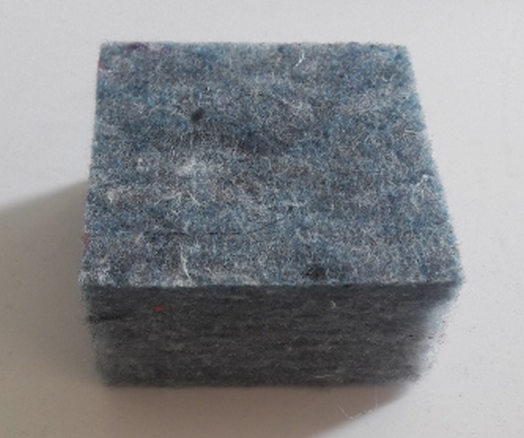
\includegraphics[width=\textwidth]{insul}
    \caption{A sample of the nonwoven textile waste insulation}
\end{marginfigure}

\par Finally TDART includes multifunctional sealing %(air-tightness, impermeability etc.)%
membranes which double as a high albedo "cool roof". Previous literature suggests significant air-conditioning energy savings can be achieved in high temperatures which are prevalent in the African climate\cite{akbari2003measured, akbari1999cooling} especially in urban heat island environments. In a 1999 study, researchers extrapolated simulation data to the US and estimated that white roofing can potentially save up to 10 \si{{\tera\watt\hour}} per year. A more recent study\cite{pisello2013active} of a typical office building in Rome, Italy found a decrease of 34\% in energy requirements for cooling. In terms of environmental impact, cool roofs have been shown to be three times more effective than green roofs at cooling the globe for climate change mitigation\cite{sproul2014economic}, making this a very attractive solution for TDART.
	\vspace*{2cm}\\
	\textcolor{orange}{\textit{\Huge{Meta-innovation through project management}}}
	\vspace*{2cm}\\

	In any project that brings together different backgrounds, disciplines and personalities, making it all run smoothely will be a challenge, as is the case for TDART. Our ultimate goal remains to expose our members to the thick of industry and sustainable construction. This experience will sharpen their skills and provide them with experience and a variety of tools that they can use in the future in order to further develop and contribute to their own fields long term, all while building an innovative net-zero energy house on the immediate term. But achieving this in a competitive context requires a bit of "meta-innovation". Considering TDART first and foremost as a prime example of project based pedagogy, our model is split into three approaches: Project, Competition and Human based.
	\begin{marginfigure}
\resizebox{\textwidth}{!}{%
  \begin{tikzpicture}
  \begin{scope}[blend group = soft light]
    \fill[red!30!white]   ( 90:1.2) circle (2);
    \fill[green!30!white] (210:1.2) circle (2);
    \fill[blue!30!white]  (330:1.2) circle (2);
  \end{scope}
  \node at ( 90:2)    {Project};
  \node at ( 210:2)   {Human};
  \node at ( 330:2)   {Competition};
  \node [font=\Large] {TDART};
\end{tikzpicture}
}
\caption{The three approaches to team management in TDART}
\end{marginfigure}
	The \textit{project} based approach rests on the idea of putting the students in the thick of industry, real-world practices and challenges with deadlines, quality requirements and budget caps. This provides them with much needed experience that will help them be more effective in similar contexts in the future.\\
	The \textit{competition} approach serves mainly to provide constant motivation to the team members. Working in a competitive context makes the students work harder to understand their abilities and how to collaborate with one another to make up a cohesive unit that works towards achieving a common goal.\\
	The \textit{Human} based approach is about task assignment according to background and ability, conflict management and team-building. We aimed to provide an environment where healthy minority dissent can help improve creativity and prevent premature consensus and encourage the majority to consider issues from different perspectives as was suggested by Nemeth\cite{nemeth1986differential} in the 80s. This requires the team to have a high level of reflexivity, which is, as defined by West\cite{west1996reflexivity}, overtly reflecting upon the team's objectives, strategies and processes and adapt them to current or anticipated circumstances.
	
	\bibliography{sample-handout}
	\bibliographystyle{plainnat}
	
\end{document}
